\documentclass[tikz,border=5pt]{standalone}
\usepackage{luatexja}
\usepackage[hiragino-pron]{luatexja-preset}
\usepackage{amsmath,amssymb,bm}
\usetikzlibrary{arrows.meta}

\begin{document}
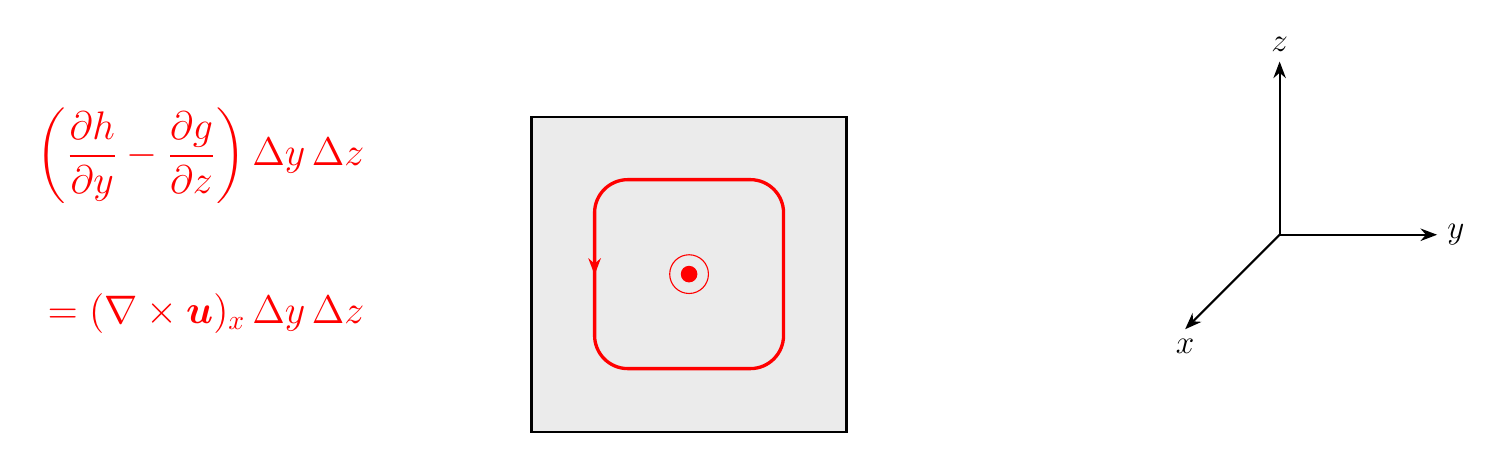
\begin{tikzpicture}[every node/.style={font=\large}]

  %% Left: formula
  \node[red, font=\Large, anchor=east] at (0,1.5) {$\left(\dfrac{\partial h}{\partial y} - \dfrac{\partial g}{\partial z}\right) \Delta y\, \Delta z$};
  \node[red, font=\Large, anchor=east] at (0,-0.5) {$= (\nabla \times \boldsymbol{u})_x\, \Delta y\, \Delta z$};

  %% Center: yz-plane (front view) with circulation
  \begin{scope}[xshift=4cm]
    % Rectangle for yz-plane
    \fill[black!8] (-2,-2) rectangle (2,2);
    \draw[thick] (-2,-2) rectangle (2,2);

    % Circulation arrow (red, clockwise)
    \draw[very thick, red, rounded corners=12pt]
      (-1.2,-1.2) -- (-1.2,1.2) -- (1.2,1.2) -- (1.2,-1.2) -- cycle;
    \draw[-{Stealth[length=6pt]}, very thick, red] (-1.2,0.0) -- (-1.2,-0.01);

    % x-component: dot (arrow coming out of plane toward viewer)
    \fill[red] (0,0) circle (3pt);
    \draw[red] (0,0) circle (7pt);
  \end{scope}

  %% Right: xyz axes
  \begin{scope}[xshift=11.5cm, yshift=0.5cm]
    \draw[-{Stealth[length=6pt]}, thick] (0,0) -- (0,2.2) node[above] {$z$};
    \draw[-{Stealth[length=6pt]}, thick] (0,0) -- (2,0) node[right] {$y$};
    \draw[-{Stealth[length=6pt]}, thick] (0,0) -- (-1.2,-1.2) node[below] {$x$};
  \end{scope}

\end{tikzpicture}
\end{document}
